\subsection{Zpracování exportovaných segmentů biosignálů}
\label{subsec:prezpracovani_segmentu}
Pro každého člena posádky byly exportovány segmenty biosignálů o délce 30s s
50\% překryvem na základě poznatků
v~\cite{Castaldo2019,Kim2021,Pecchia2018,Shaffer2020,Tervonen2021}. Zpracování
biosignálu vycházelo z metodiky popsané v sekci~\ref{sec:zpracovani_biosignalu}.
U každého segmentu proběhlo hodnocení jeho kvality podle dvou kritérií:
\begin{itemize}
      \item Hodnocení kvality \gls{EKG} signálu pomocí heuristické fúze a fuzzy
            komplexního hodnocení podle~\cite{Zhao2018}.
      \item Hodnocení detekovaných R vln z hlediska časové kontroly náhlých
            nefyziologických změn v po sobě jdoucích R-R intervalech.
\end{itemize}
Segmenty, které vykazovali nežádoucí anomálie v rámci hodnotících kritérií, byly
vyřazeny. Ze segmentů bylo dále vypočteno přes 100 různých parametrů pro účely
analýzy dat. Mezi tyto parametry patřily například běžné statistické
charakteristiky (průměr, medián, směrodatná odchylka a další), nelineární a
časové \gls{HRV} parametry. Dále byly identifikovány a označeny úseky v časech
kognitivních testů. Z časových důvodů nebyly pro účely této práce ostatní
aktivity během mise anotovány, i přes dostupnost kamerových záznamů. Seznam
všech počítaných parametrů je součástí přílohy v souboru
\texttt{all\_params.csv}. 

\subsection{Čistění dat}
\label{subsec:cisteni_dat}
Ze souborů vypočtených parametrů byly vynechány všechny parametry, jejichž
sloupce obsahovali \texttt{NaN} hodnoty. Dále byly parametry korelovány a
odstranily se ty, které byly vzájemně dokonale korelované ($|r| > 0,999$). Poté
se odstranily odlehlé hodnoty na základě absolutní odchylky mediánu (MAD) od
mediánu.

\subsection{Sledované veličiny}
\label{subsec:sledovane_veliciny}
Pro účely analýzy \gls{NPF} adaptace subjektů v průběhu mise byly na
základě~\cite{Pereira2017,Shaffer2017} vybrány a sledovány především následující
\gls{HRV} parametry:
\begin{itemize}
      \item \textbf{SD2} --- Směrodatná odchylka Poincarého grafu podél přímky
      totožnosti.
      \item \textbf{RMSSD} --- Odmocnina ze středního kvadratického rozdílu mezi
            po sobě následujícími N--N intervaly.
      \item \textbf{pNN50} --- Procento po sobě následujících N--N intervalů,
            které se od sebe liší o více než 50~ms.
      \item \textbf{HF} --- Vysokofrekvenční složka výkonu variability srdeční
            frekvence.
\end{itemize}
Průběhy jednotlivých sledovaných veličin během analogové vesmírné mise DIANA
jsou vizualizovány na Obr.~\ref{fig:params_example}.

\begin{figure}[H]
      \begin{center}
            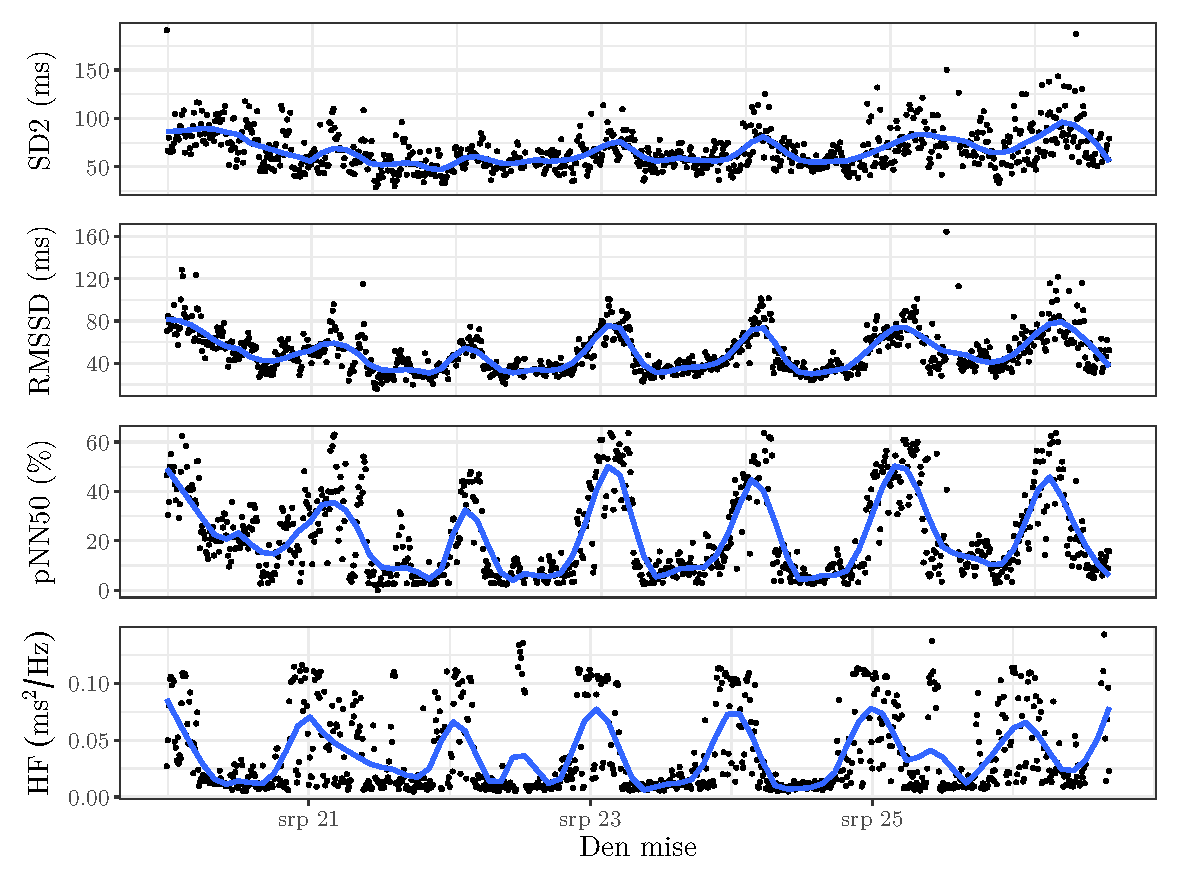
\includegraphics[width=1\linewidth]{figures/stats/hourly_params.pdf}
            \caption{Příklad průběhu sledovaných veličin během mise. Jedná se o
             agregované hodnoty mediánem za každých 10 minut. Data jsou
             proložena využitím loess regrese ($\alpha = 0,01$).}
            \label{fig:params_example}
      \end{center}
\end{figure}

\subsection{Analýza dat mise}
\label{subsec:analyza_diana}
Vzhledem k nereprezentativnosti a nepopsanosti dat byly primárně pro potřeby
jejich analýzy namísto statistických testů a dalších nástrojů použity zejména
vizuální metody. Pro zobrazení denního vývoje v rámci sledovaných parametrů byly
vypočtené parametry agregovány mediánem na úrovní hodin i dnů. Vizualizace byla
v tomto případě spojena i s výsledky statistického modelování popsaného v
následující sekci. Pro účely vizuální analýzy byly použity krabicové grafy.

Dále byly identifikovány, exportovány a vizualizovány segmenty biosignálů v
časech, kdy subjekt vykonával \gls{NPF} baterii testů. Segmenty byly
vizualizovány využitím krabicových grafů. Výsledky v rámci vizuálních analýz se
nacházejí v sekci~\ref{sec:vysledky_vizual} a dále jsou probírány v samotné
diskuzi.

\subsection{Statistické modelování}
\label{subsec:tvorba_modelů}
Ke zkoumání vztahu mezi vybraným sledovaným parametrem napříč jednotlivými dny v
rámci obou skupin, mateřské lodi a přistávacího modulu, byl vytvořen
víceúrovňový lineární smíšený model. Nechť $Y$ je vektor odezvy (tj.
\enquote{vybraný sledovaný parametr}). Po zahrnutí interakce dnů a skupin lze
lineární smíšený model zjednodušeně a vektorově vyjádřit následovně:
\begin{equation}
      Y = \beta_{0}+\beta_{1} {d}+\beta_{2} {s}+\beta_{3} {d} {s} + u_{0} + u_{1}d + \epsilon, \quad \epsilon \sim \mathcal{N}\left(0, \sigma^2\right)
\end{equation}
kde $\beta_i$ jsou vektory koeficientů fixních efektů, $\epsilon$ je člen
reziduální chyby a $d, s$ označují fixní efekty den a skupinu. Náhodné efekty
jsou označeny jako $u_0, u_1$. Dále je přítomna zmíněna interakce v podobě
zahrnutí interakčního členu $d \cdot s$. To znamená, že kromě samostatného
modelování vlivu \enquote{dne} a \enquote{skupiny} model zohledňuje také
případnou interakci mezi nimi. Jinými slovy, model počítá s možností, že vliv
\enquote{dne} na proměnnou odezvy (závislou proměnnou) se může lišit v
závislosti na úrovni \enquote{skupiny}. Zároveň díky zvoleným náhodným efektům
je v rámci dnů dovoleno individuálním rozdílům na úrovni subjektů. V případě
všech navržených modelů byla také analyzována i jejich síla. Jelikož bývá
obtížné přesně určit sílu smíšeného modelu pomocí tradičních statistických
metod, byla zvolena simulace, která je často účinnějším a preferovanějším
přístupem~\cite{Green2016}. Konkrétně byla zvolena Monte Carlo simulace pro svou
flexibilitu a přesnost~\cite{Bolker2008,Johnson2015}. Simulace je součástí
přílohy v podobě skriptu s názvem \texttt{MC\_Simulation.R}.

Výsledky modelování jsou uvedeny v sekci~\ref{sec:vysledky_lmm} a rozebrány v
diskuzi. Modelování bylo realizováno v programovém jazyce R. Vzhledem k tomu, že
se lineární smíšené modely řadí mezi statistické metody, tak jsou samostatně
popsány v sekci~\ref{sec:statisticke_metody}.